\def\QRCODE{MASTER_mispa_TUT.IMG.morphological_attribute_filtering_matlabqrcode.png}
\def\QRPAGE{http://www.iptutorials.science/tree/master/MASTER_mispa/TUT.IMG.morphological_attribute_filtering/matlab}
\mcorrectionsection{Matlab correction}

\subsection{Binary attribute filtering}
If $I$ is a binary image, the different attribute are proposed in the following code (filtering small squares -- $25\times 25$, small objects, by elongation or convexity, respectively).

\begin{matlab}
S= imreconstruct(imopen(I,strel('square',25)), I));
A= bwareaopen(I, 1000);
E= bwpropfilt(I, 'eccentricity', [0.75 1]);
C= bwpropfilt(I, 'solidity', [0.75 1]);
\end{matlab}

\subsection{Grayscale filtering}
The grayscale filtering is the previous binary filtering process applied to all level-sets of the original image. The image is first decomposed into the level-sets.

\begin{matlab}
A = double(imread('toy.png'));
A = A(:,:,1);

%% IMAGE DECOMPOSITION
[m,n] = size(A);
levelSets_init = false(m,n,256);
for s=0:255
    levelSets_init(:,:,s+1) = A>=s;
end
\end{matlab}

Then, for each level, the binary set is filtered by some attribute, and the resulting image is reconstructed by taking the maximum value on all levels.
\begin{matlab}
%% ATTRIBUTE FILTERING
levelSets_res1 = zeros(m,n,256);
levelSets_res2 = zeros(m,n,256);
levelSets_res3 = zeros(m,n,256);
levelSets_res4 = zeros(m,n,256);
for s=0:255
    levelSets_res1(:,:,s+1) = s*(imreconstruct(imopen(levelSets_init(:,:,s+1),strel('square',25)),levelSets_init(:,:,s+1)));
    levelSets_res2(:,:,s+1) = s*bwareaopen(levelSets_init(:,:,s+1),1000);
    levelSets_res3(:,:,s+1) = s*bwpropfilt(levelSets_init(:,:,s+1),'eccentricity',[0.75 1]);
    levelSets_res4(:,:,s+1) = s*bwpropfilt(levelSets_init(:,:,s+1),'solidity',[0.75 1]);
end

%% IMAGE RECONSTRUCTION
B1 = max(levelSets_res1,[],3);
B2 = max(levelSets_res2,[],3);
B3 = max(levelSets_res3,[],3);
B4 = max(levelSets_res4,[],3);
\end{matlab}

Results are illustrated in 
\iflabelexists{fig:morphological_attribute_filtering:enonce:examples}%
{Fig.\ref{fig:morphological_attribute_filtering:enonce:examples}.}%
{Fig.\ref{fig:morphological_attribute_filtering:matlab:examples}.
\begin{figure}[htbp]
\centering

\subfloat[Filtering by area.]{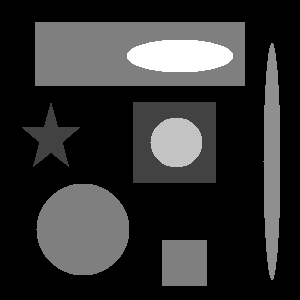
\includegraphics[width=.2\linewidth]{toy_areaOpening.png}}\hfill
\subfloat[Filtering by elongation.]{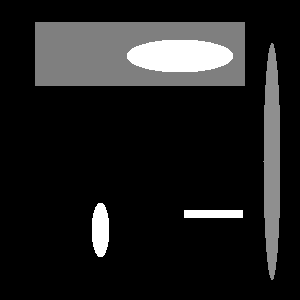
\includegraphics[width=.2\linewidth]{toy_elongThinning.png}}\hfill
\subfloat[Filtering by con\-ve\-xi\-ty.]{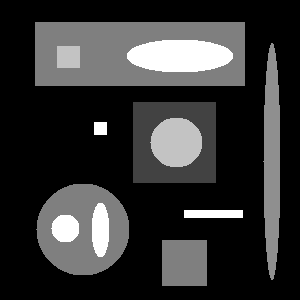
\includegraphics[width=.2\linewidth]{toy_convThinning.png}}\hfill
\subfloat[Filtering objects larger than a square.]{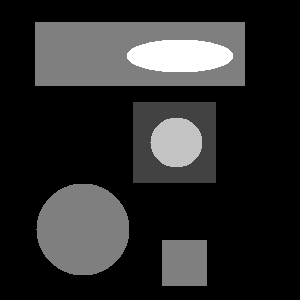
\includegraphics[width=.2\linewidth]{toy_recOpening.png}}

\caption{Attribute filtering examples.}
\label{fig:morphological_attribute_filtering:matlab:examples}
\end{figure}
}%
